\chapter{Analiza otrzymanych wyników}
\label{cha:analiza_otrzymanych_wynikow}


\section{Analiza działania użytych algorytmów}

W celu implementacji algorytmu wyszukania optymalnych tras, w aplikacji została zaimplementowana obsługa kilku algorytmów wyszukiwania ścieżek w grafie. Standardowo aplikacja korzysta tylko z jednego z nich, implementacja ma na celu tylko ich porównanie. W poniższych akapitach przedstawiono testy porównawcze prędkości działania algorytmów podczas wyznaczania tras pomiędzy zestawem wybranych losowo punktów na mapie Krakowa. 
W celu heterogenizacji wyznaczonych tras, punkty początkowe i końcowe każdej z nich zostały dobrane w taki sposób aby pokryły odpowiedni obszar Krakowa a także przebiegały w miejscach gęsto i luźno obstawionych przez ścieżki zawarte w posiadanym zbiorze danych. Z tego powodu niektóre z nich przebiegają w okolicach rynku, a inne przez Wolę Justowską gdzie jedyną ścieżką w posiadanym zbiorze jest droga po wale rzeki Rudawy.
Obydwa z zaimplementowanych algorytmów gwarantują każdorazowo wyznaczenie optymalnej trasy, nie kończą przeszukiwania po uzyskaniu pierwszej znalezionej trasy, stąd porównanie można uznać za miarodajny wynik złożoności obliczeniowej każdego z algorytmów.

\subsection{Porównanie działania algorytmu z wykorzystaniem algorytmu Dijkstra i A*}

Na poniższym wykresie zestawiono czasy działania obydwu algorytmów wraz z opisem trasy dla której każdy z czasów został wyznaczony.

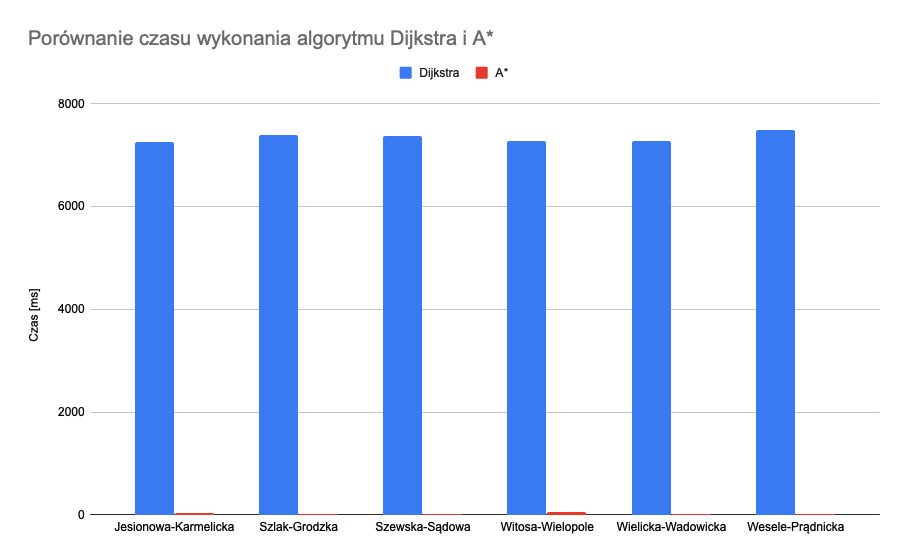
\includegraphics[width=\textwidth]{czas_dijkstra_vs_a}

Z wykresu można odczytać że algorytm A* sprawdza się nieporównywalnie lepiej w stosunku do algorytmu Dijkstra w kontekście czasu wykonania. Z wykresu ciężko nawet odczytać różnice w czasie działania ze względu na minimalny wkład czasów osiągniętych przez A*. W najgorszym z zaprezentowanych przypadków jego działanie było około 200 krotnie szybsze, w najlepszym z przypadków różnica w prędkości działania była prawie 500 krotna. Z powyższego zestawienia jasno wynika, że do produkcyjnego zastosowania w aplikacji w porównaniu z algorytmem Dijkstra nadaje się tylko algorytm A*. Jest on za to znacznie bardziej czasochłonny w implementacji, stąd jego zastosowanie do zdecydowanie mniej złożonych grafów może być korzystniejsze. W celu zminimalizowania czasu wykonywania algorytmu Dijkstra można było zastosować odpowiednie zmniejszenie grafu na podstawie filtracji wierzchołków które znajdują się wewnątrz obszaru na mapie zawartego przez punkt końcowy i początkowy. Jednak ze względu na brak potrzeby optymalizacji i odpowiednią wizualizację różnic czasu działania zaniechano tej modyfikacji.
W przypadku przeszukania grafu w którym wierzchołki mogą być określone jako punkty na mapie, algorytm A* jest zdecydowanie szybszy ze względu na prostotę wyznaczenia heurystyki. W tym wypadku przewidywanie czy droga zbliża się do końca może być określone przez wyznaczenie odległości pomiędzy ma złożoność obliczeniową O(1) i polega na wyznaczeniu odległości pomiędzy kolejnym sprawdzanym wierzchołkiem a punktem końcowym trasy. Dzięki temu, w przeciwieństwie do algorytmu Dijkstra, A* nie prowadzi przeszukania całego grafu przed wyznaczeniem optymalnej ścieżki a ogranicza się jedynie do przeszukania szeregu dróg które prowadzą pomiędzy punktem końcowym i początkowym.
Ogólną złożoność obliczeniową algorytmu A* przedstawiono poniższym wzorem.

// tutaj wzór na złożoność ogólną A*

Dla przykładu algorytmu użytego w aplikacji może zostać wyznaczona wzorem:

// tutaj wzór na złożoność A* w tym przypadku.

Na podstawie wzoru widać że złożoność algorytmu A* w dużej mierze zależy od złożoności obliczeniowej wyznaczenia heurystyki. W przypadku gdy proces ten przedstawiał by się złożonością obliczeniową O(n2), algorytm działał by z prędkością porównywalną do algorytmu Dijkstra.

\subsection{Czas działania algorytmu A* i Dijkstra w zależności od długości trasy}

Na poniższych wykresach przedstawiono czas działania algorytmu A* i Dijkstra w zależności od obszaru objętego przeszukiwaniem. W tym celu na terenie Krakowa wyznaczono zestaw tras w zakresie od bardzo krótkich, obejmujących tylko kilkaset metrów do takich obejmujących teren całego Krakowa.

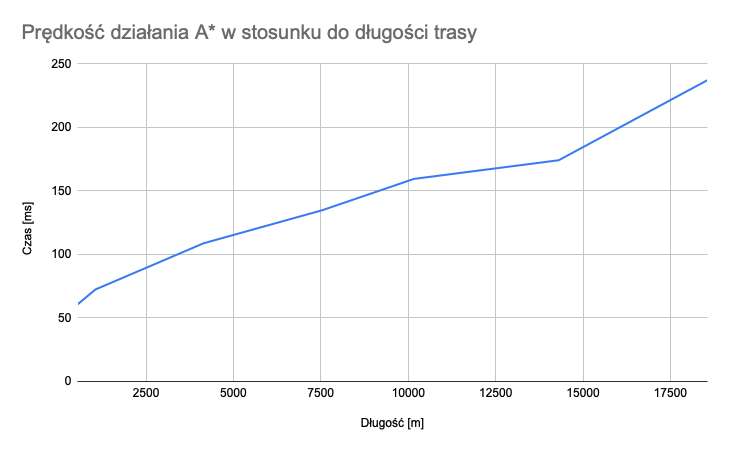
\includegraphics[width=16cm]{a_a_dlugosc_trasy}

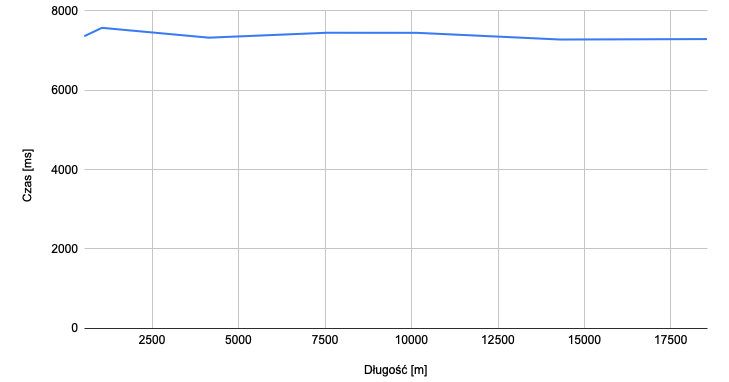
\includegraphics[width=16cm]{dijkstra_a_dlugosc_trasy}

Z przedstawionych wykresów można odczytać że czas działania algorytmu Dijkstra nie zależy od długości wyznaczonych tras. Delikatne fluktuacje czasu wykonania zależą od aktualnego użycia pamięci i procesora komputera podczas wykonywania testu. Jest to spowodowane zasadą działania algorytmu Dijkstra, który w każdym przypadku w pierwszej kolejności wykonuje obliczenia najkrótszych ścieżek pomiędzy wszystkimi wierzchołkami grafu.
Przeciwny przypadek obowiązuje dla algorytmu A* który dzięki zastosowaniu heurystyki jest w stanie wykryć gdy najkrótsza ścieżka została już odnaleziona i zatrzymać przeszukiwanie w odpowiednim przypadku. Z tego powodu w zależności od obszaru grafu obejmowanego przez przeszukanie, algorytm A* wykazuje znaczny, liniowy wzrost czasu wykonania.

\subsection{Porównanie algorytmu zachłannego A* i standardowej implementacji A*}

Kolejnym etapem analizy jest określenie czasu oraz jakości działania algorytmu zachłannego A* w stosunku do podstawowej wersji A*. W przeciwieństwie do standardowej implementacji, algorytm zachłanny, zyskując na czasie wykonania, nie gwarantuje wyznaczenia optymalnej ścieżki pomiędzy wierzchołkiem początkowym i końcowym. Bazując na przekazanej heurystyce, stara się wyznaczyć najlepsze lokalne rozwiązania podzbiorów składających się na wynikową trasę, następnie łączy uzyskane podzbiory w celu wyznaczenia trasy. W poniższych akapitach zawarto analizę czasu wykonania oraz wyznaczonych wag tras w zależności od typu algorytmu.
Na poniższym wykresie przedstawiono zestawienie wag tras wyznaczonych przez obydwa algorytmy dla uprzednio wyznaczonego zestawy ścieżek testowych.

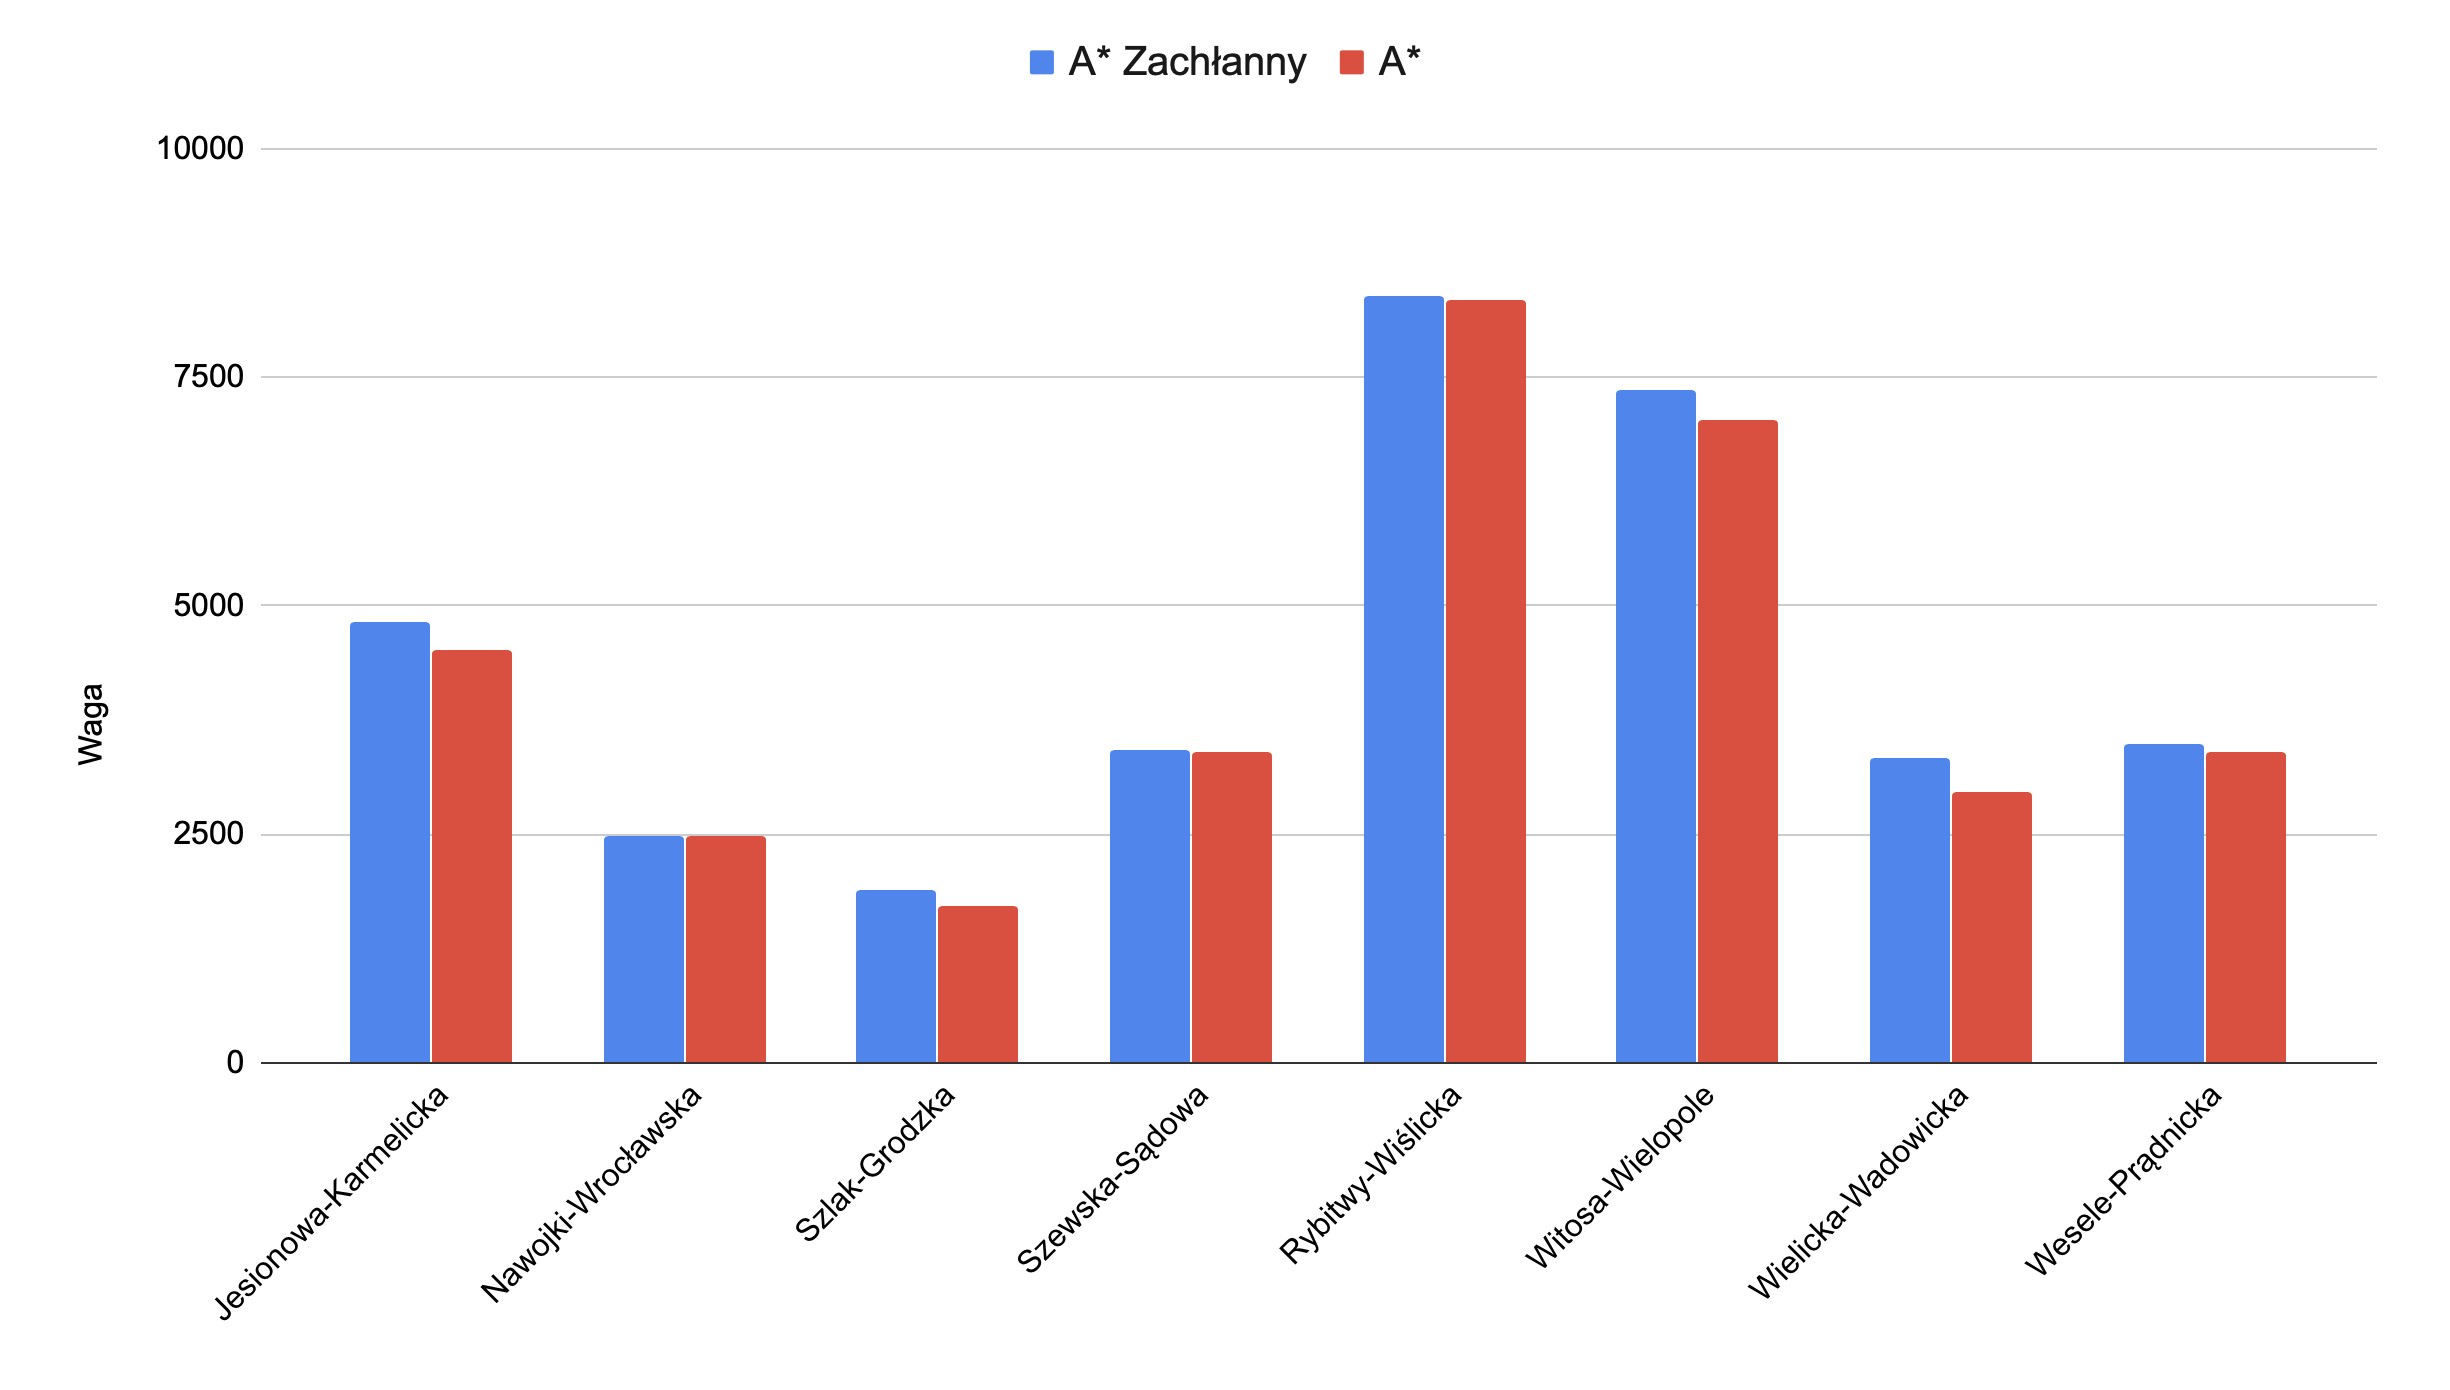
\includegraphics[width=\textwidth]{waga_a_vs_a_greedy}

Korzystając z wartości przedstawionych na powyższym wykresie można odczytać że poza przypadkiem bardzo krótkiej drogi pomiędzy ulicami Nawojki i Wrocławską, zachłanna odmiana algorytmu A* w każdym wypadku wyznaczyła trasę która z punktu widzenia waga jest gorsza niż ta wyznaczona przez standardową odmianę algorytmu A*.

Na poniższym wykresie przedstawiono zestawienie czasu działania dla uprzednio wyznaczonego zestawu testowych ścieżek.

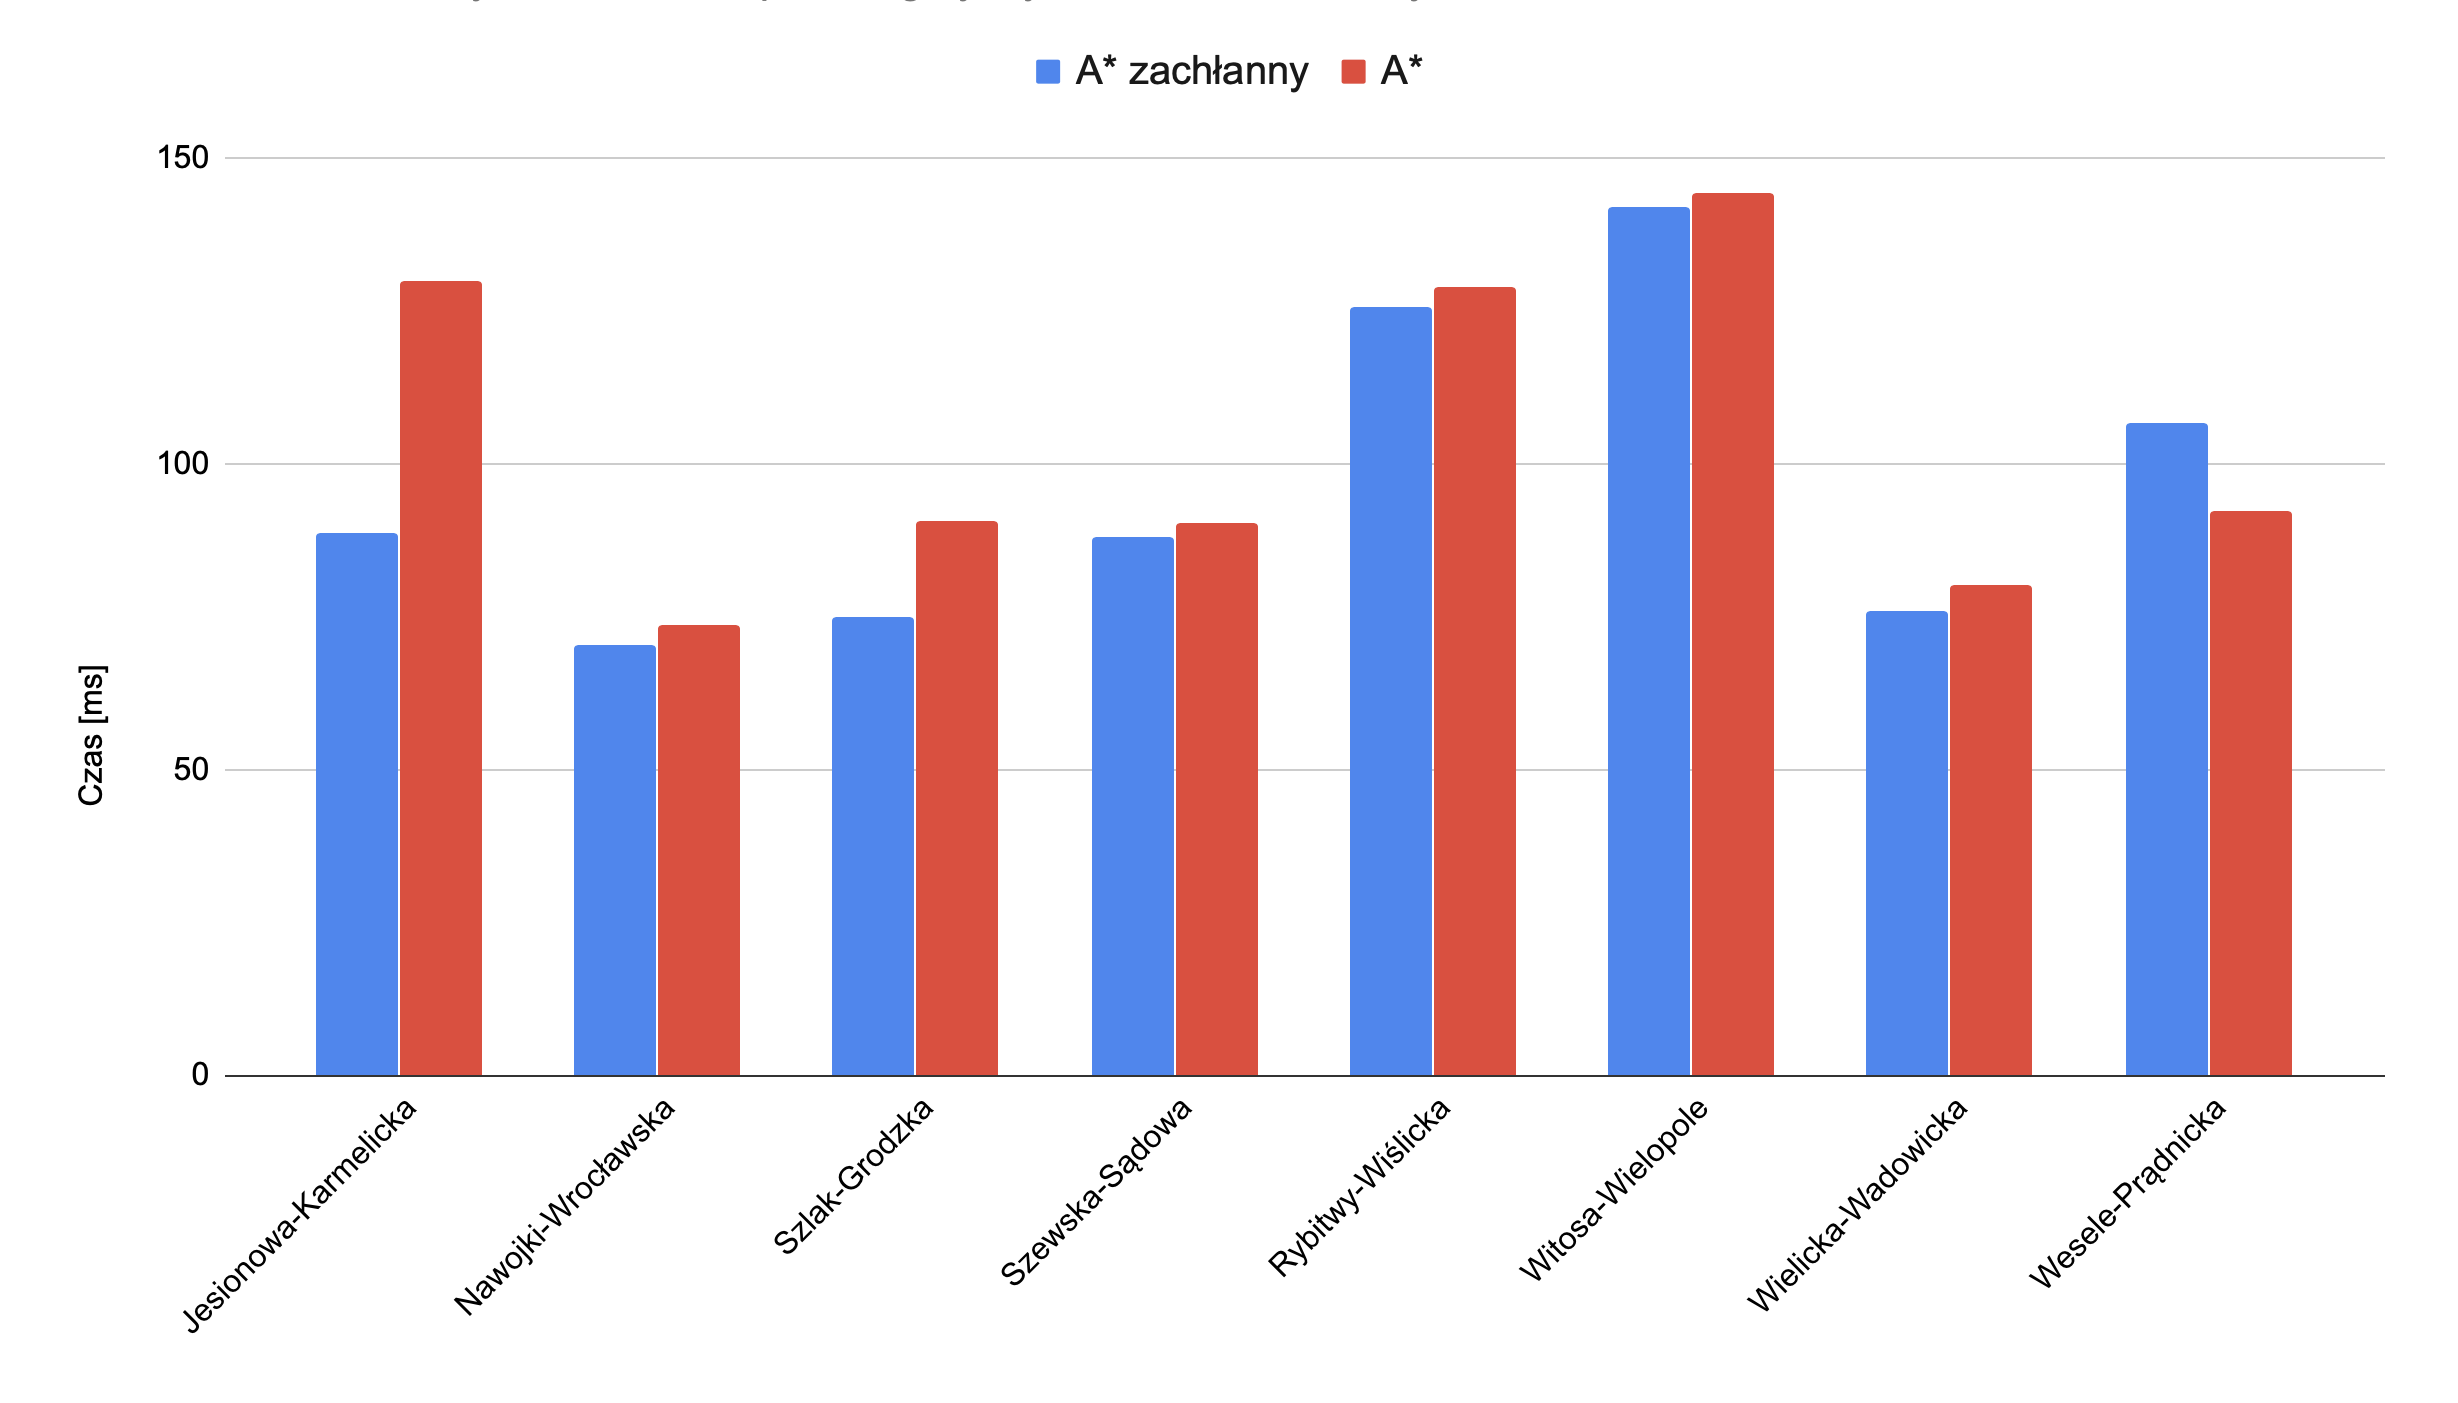
\includegraphics[width=\textwidth]{czas_a_vs_a_greedy}

Za wyjątkiem jednego przypadku, który może być spowodowany chwilową mniejszą wydajnością maszyny na której działały testy, algorytm zachłanny uzyskał lepszy średni czas wyznaczania trasy. Jest to spodziewane, ponieważ algorytm ten w swojej zasadzie działania stara się optymalizować czas wykonania kosztem jakości. Różnice w czasie działania dla większości przypadków są bardzo niewielkie, sumując je z brakiem gwarancji wyznaczenia trasy optymalnej, algorytm zachłanny A* nie znajduje zastosowania do użycia w stworzonym algorytmie.

\subsection{Porównanie algorytmu NBA i standardowej implementacji A*}

W celu dalszej analizy możliwych usprawnień dla czasu działania algorytmu, został zaimplementowany i porównany także algorytm NBA*(New Bidirectional A*). Jest to odmiana algorytmu A* który w celu optymalizacji czasu działania jednocześnie rozpoczyna swoje wykonywanie z punktu końcowego do punktu początkowego oraz w przeciwną stronę. Złożoność obliczeniowa wykonania obydwu algorytmów pozostaje taka sama, jednak istnieje możliwość wykonywania dwóch algorytmów przy wykorzystaniu dwóch rdzeni procesora, dzięki czemu czas obliczeń ulega znacznej poprawie. W przeciwieństwie do algorytmu zachłannego, algorytm NBA gwarantuje każdorazowe wyszukanie optymalnej trasy w grafie.
Na poniższym wykresie przedstawiono zestawienie czasów działania algorytmów. W celu otrzymania porównywalnych wyników, porównania zostały także przeprowadzone dla tego samego zestawu danych testowych.

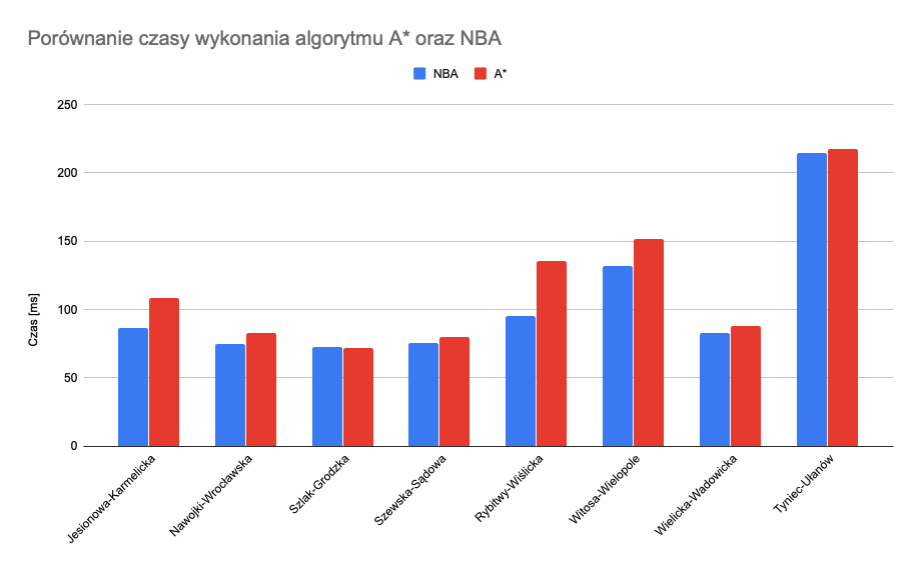
\includegraphics[width=\textwidth]{czas_a_vs_nba}

Z uzyskanych wyników można odczytać że algorytm NBA daje możliwość uzyskania nieznacznie mniejszych czasów obliczeń. Same różnice nie są duże, ale znikomym nakładem pozwalają nieznacznie obniżyć wykorzystanie zasobów serwera w przypadku gdy aplikacja jest używana przez znaczną ilość ludzi. Z wykresu można także odczytać nieznaczny trend w kierunku zwiększenia różnic wykonania algorytmu w przypadku gdy trasy są dłuższe. Jest to spowodowane faktem że zasoby czasowe potrzebne na alokację oraz rozpoczęcie procedury przeszukiwania grafu z obydwu stron mogą być skompensowane przez rzeczywisty zysk uzyskany przez samą procedurę przeszukiwania. Czas obliczeń dla tras o długości 800-2000m jest w przypadku obydwu algorytmów prawie taki sam.

\section{Porównanie wyników w stosunku do tras wyznaczonych przez Google Maps}